%!TEX root = ../report.tex

\begin{document}
\chapter{Notes/Remarks}

\section{Related work - Datasets}
%Since the advent of AlexNet \cite{alexnet}, deeplearning has been in the rise. 
%Deep convolutional neural networks are the desired option for image analysis tasks such as classification, detection and segmentation.
%These deep convolutional networks are successful especially because of two reasons. 
%First is the architectures and their paralellisation, allowing them to train millions of images on a GPU.
%Second reason is the development of huge public benchmark datasets such as Imagenet \cite{imagenet}, Pascal VOC \cite{pascalvoc} and COCO \cite{coco} datasets
%Although deep convolutional networks are huge success in image analysis tasks, they perform poorly on 3D point cloud data.
LiDAR is one of the central component in the sensor suite for SLAM system in robotic applications \cite{thrun2006stanley}, \cite{patz2008practical}, \cite{hess20162dSLAM} and autonomous driving \cite{li2016vehicle}.
3D LiDAR data is preferred because, it can provide the exact replica of 3D geometry of the real world represented in the form of 3D point clouds.
Because of these rich features and widespread use of LiDAR sensors, tasks such as 3D object detection \cite{zhou2018voxelnet}, \cite{PIXOR} and 3D semantic segmentation \cite{qi2017pointnet++}, \cite{3Dmininet} are becoming more predominant area for research.

In this section, we will discuss about the available 3D LiDAR datasets for 3D semantic segmentation task and classify the datasets based on acquisition methods as in \cite{survey3d}.
\cite{survey3d} classifies the available public datasets into three classes based on the data acquisition process.
They are \textit{Sequential}, \textit{Static} and \textit{Synthetic} datasets.
The data for sequential datasets are collected as frame sequences where mechanical LiDAR is mounted on top of a autonomous driivng platform as in Figure \ref{fig:seq_data_lyft}.
\begin{figure}[h!]
    \centering
    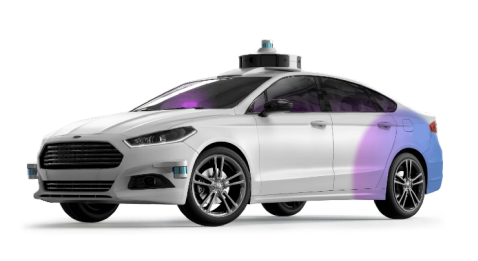
\includegraphics[scale=0.25]{images/sequential_lyft.png}
    \caption{Sequential mounted LiDAR for data collection of Lyft L5 dataset. Image from \cite{Lyftl5}}
    \label{fig:seq_data_lyft}
\end{figure}
Most of the popular autonomous driving datasets are of sequential type, but these kind of datasets comes with a drawback of sparse points than other datasets.

Static datasets consists of data collected from a stationary view point by a terrestrial laser scanner.
These kind of datasets capture the static information of the realworld whereas the sequential datasets capture the dynamic movements of the surrounding objects.
Static datasets find their way in applications such as the urban planning, augmented reality and robotics. 
Figure \ref{fig:tls} depcits a terrestrial laser scanner used to capture point cloud of an industrial environment.
\begin{figure}[h!]
    \centering
    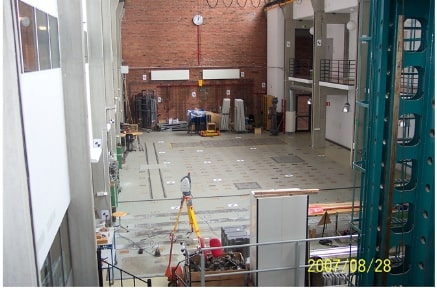
\includegraphics[scale=0.75]{images/TLS.jpg}
    \caption{Terrestrial laser scanner in an industrial environment with the laser scanner mounted on a yellow tripod in the left corner of the floor. Image taken from \cite{tls}}
    \label{fig:tls}
\end{figure}
An advantage with the static datasets, are they can produce highly dense point clouds leading to rich 3D geometric representations.

Last type of 3D LiDAR datasets are synthetic datasets. 
As the name suggests these datasets are generated from the computer simulation. 
Figure \ref{fig:synthetic} depcits a simulated point cloud in a synthtic dataset called SynthCity.
Eventhough synthetic datasets can be generated in large scale with cheap cost, they lack the accuracy in detail when compared to the point clouds generated from real world.
\begin{figure}[h!]
    \centering
    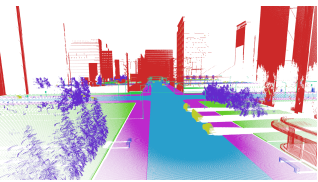
\includegraphics[scale=0.5]{images/synthcity.png}
    \caption{Illustration of a scene in synthetic dataset called SynthCity. Image taken from \cite{griffiths2019synthcity}}
    \label{fig:synthetic}
\end{figure}
\section{TODO}
\begin{itemize}
    \item[$\bullet$] Add the table for the dataset and explain the table
    \item[$\bullet$] Add the mindmap for better visualization
    \item[$\bullet$] Discuss why SemanticKITTI and Semantic3D are of our interest     
\end{itemize}
\end{document}
